% Chapter Template

\chapter{Technologies, Toolchain and Hardware} % Main chapter title

\label{Technologies, Toolchain and Hardware} % Change X to a consecutive number; for referencing this chapter elsewhere, use \ref{ChapterX}

%----------------------------------------------------------------------------------------
%	Hardware, Technologies, Toolchain and Programming Languages
%----------------------------------------------------------------------------------------

\section{Technologies and Programming Languages}
Software is a generic term for organized collections of computer data and instructions, often broken into two major categories: system software that provides the basic non-task-specific functions of the computer, and application software which is used by users to accomplish specific tasks.
\newline

System software is responsible for controlling, integrating, and managing the individual hardware components of a computer system so that other software and the users of the system see it as a functional unit without having to be concerned with the low-level details such as transferring data from memory to disk, or rendering text onto a display. Generally, system software consists of an operating system and some fundamental utilities such as disk formatters, file managers, display managers, text editors, user authentication (login) and management tools, and networking and device control software.
\newline

Application software, on the other hand, is used to accomplish specific tasks other than just running the computer system. Application software may consist of a single program, such as an image viewer; a small collection of programs (often called a software package) that work closely together to accomplish a task, such as a spreadsheet or text processing system; a larger collection (often called a software suite) of related but independent programs and packages that have a common user interface or shared data format, such as Microsoft Office, which consists of closely integrated word processor, spreadsheet, database, etc.; or a software system, such as a database management system, which is a collection of fundamental programs that may provide some service to a variety of other independent applications.
\newline

Software is created with programming languages and related utilities, which may come in several of the above forms: single programs like script interpreters, packages containing a compiler, linker, and other tools; and large suites (often called Integrated Development Environments) that include editors, debuggers, and other tools for multiple languages.[\cite{6}] 
\newline

\subsubsection*{Programming Languages}
There exists an enormous variety of programming languages in use today. Testimony of this fact are the 650 plus different programming languages listed in Wikipedia [\footnote{\href{http://en.wikipedia.org/wiki/List\_of\_programming\_languages}{\texttt{List of programming languages}}}]. A good understanding of this great diversity is important for many reasons. First, it opens new perspectives to the computer scientist. Problems at first hard in one language might have a very easy solution in another. Thus, knowing which language to use in a given domain might decrease considerably the effort to build an application.


\subsubsection*{What is a Programming Languages}
A programming language is an artificial language that can be used to instruct a computer to do a particular task. To be considered a general programming language, it must be computationally complete, or Turing-Complete. It is nevertheless common to regard some languages that are not computationally complete, like database query languages and other domain-specific languages as programming languages as well.

\subsubsection*{High-Level Versus Low-Level Programming Languages}

A low-level programming language is one that is very basic and close to the machine's native language. A low-level programming language can be thought of as a building block language for software. Assembly code is the most common low-level language and requires very little translation to assemble it to machine code. (The 1's and 0's that make up binary.)[\cite{6}]
\newline

A high-level programming language is one that is closer to a level of human communication. In this method, the compiler does a lot more of the work for the programmer. The closer the language is to our everyday speech, the easier it is to worry about more complex problems. However, this can be taken too far. If a language is too much like English (or other natural languages), it can be harder to create complex programs. This is because verbose languages take more time to read, and so they can take a lot more time to understand.[\cite{6}]
\newline

Machine code is the language the computer can understand directly. Machine code consists of sequences of binary digits. It is almost never programmed in directly, but anything that is to be run on an ordinary computer must be translated to machine code first. The machine code can be different for each computer architecture.[\cite{6}]
\newline

Assembly language is a more human readable representation of the machine code, where the machine instructions are represented as mnemonics rather than binary digits. Assembly language has a 1:1 relationship with machine code as long as the program is not self-modifying. Before an assembly program can be run by a computer, it must be transformed to machine code. A program that does this translation is known as an assembler. In the early days of computing, assembly language was extensively used, but today it is mainly used for very time critical parts of programs, the core of operating systems, as well as in very small computers, like the chip on a smartcard.[\cite{6}]
\newline

Machine code and assembly language are called first and second generation programming languages respectively. A programming language that has arithmetic expressions, looping constructs, functions, and other constructs that save the programmer from dealing with the machine instructions directly is known as a third-generation programming language.[\cite{6}]
\newline

High-level, domain-specific programming languages were earlier often mentioned as fourth-generation languages, while expert systems were called fifth-generation programming languages. In later years this distinction has blurred, as many very high-level general purpose programming languages like Python, Haskell and Common Lisp have emerged. Expert systems are in very little use today.[\cite{6}]

\begin{figure}[h!]
	\centering
	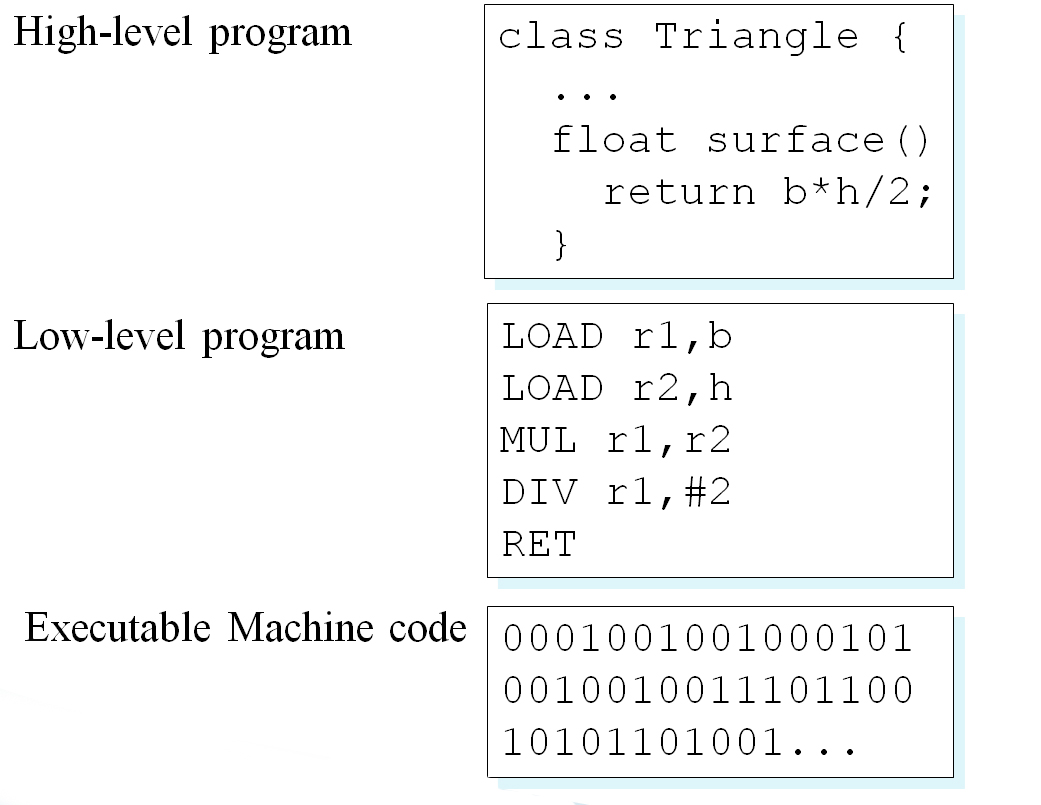
\includegraphics[width=0.7\textwidth]{./images/lavels.jpg}
	\rule{0.7\textwidth}{1pt}
	\caption{Levels of Programming Languages}
\end{figure}
\subsubsection*{Compilation and interpretation of computer programs}

Before a program can be executed on a computer, it must be translated to machine code. Alternatively it can be simulated by another program, called an interpreter. A compiler is a program that translates a programming language, called the source programming language into another programming language, called the destination language. Usually the source language is a high level language, while the destination language is machine code. An interpreter may require that the source programming language be compiled into an intermediate form before interpretetion, called byte code. This is a more low level language, for which it is easier to write an interpreter. In the Java programming language this is a separate step, while in other cases it is performed as an integral part of the interpreter. Examples of such programming languages are Perl and Python. CommonLisp is an exception to the above: it's both interpreted and compiled.[\cite{6}]

\subsubsection*{Type Systems}
There are two axes to type systems: Dynamic versus Static on the one side and Strong versus Weak.

\begin{itemize}
	\item A Strongly typed language will not allow an operation on an object if this object does not match in type. Examples are CommonLisp, Q-base and Python.
	\item A Weakly typed language will allow such operations. Examples are C and C++.
	\item TDynamic type languages bind type to value. Staticly typed languages bind it to variable.
\end{itemize}

\section*{This Software}

The software has three parts the backend, the frontend and the daemon, they communicate with each other throw a REST api[\footnote{\href{https://en.wikipedia.org/wiki/Representational\_state\_transfer}{\texttt{https://en.wikipedia.org/wiki/Representational\_state\_transfer}}}] (Figure \ref{fig:iothcomponentdiagram5}). So I will present them separately. 
\newline

In software engineering, the terms "front end" and "back end" are distinctions which refer to the separation of concerns between a presentation layer and a data access layer respectively.
\newline

The front end is an interface between the user and the back end. The front and back ends may be distributed amongst one or more systems.
\newline

In software architecture, there may be many layers between the hardware and end user. Each can be spoken of as having a front end and a back end. The front is an abstraction, simplifying the underlying component by providing a user-friendly interface.
\newline

In software design, for example, the model-view-controller architecture provides front and back ends for the database, the user and the data processing components. The separation of software systems into front and back ends simplifies development and separates maintenance. A rule of thumb is that the front (or "client") side is any component manipulated by the user. The server-side (or "back end") code resides on the server. The confusion arises when one must make front-end edits to server-side files. Most HTML designers, for instance, don't need to be on the server when they are developing the HTML; conversely, the server-side engineers are, by definition, never on anything but a server. It takes both to ultimately make a functioning, interactive website.

\begin{figure}[h]
	\centering
	\includegraphics[width=0.7\linewidth]{uml/iothcomponent}
	\caption{Iot Healthcare: Component Diagram}
	\label{fig:iothcomponentdiagram5}
\end{figure}

\subsection*{A Brief History of the Internet and the World Wide Web}
Devices are connected to it. However, the Web and its underlying Internet infrastructure had a
very different childhood that betrays the consumer and commercial base it has today.
The Internet has its roots in the U.S. Department of Defense Advanced Research Project Agency
(ARPA) project begun in or around 1960. Among the project’s goals was the ability to network
computers quickly and across great distances. The network was to be designed to be almost
fail-safe, enabling connected computers to continue communicating even if assorted routes
between them were to fail.[\cite{7}]
\newline

In 1969, the ARPANet was born, connecting several key universities. The network continued
to grow, with more and more universities coming online. One of the goals of the initial
project — robust, nearly fail-safe performance — was realized via the Internet Protocol (IP).
This protocol enabled communication packets to find various routes to a destination in case one
or more of the routes became unstable. This communication protocol became the backbone of
today’s Internet, and is how the Internet got its name.[\cite{7}]
\newline

The Transmission Control Protocol was joined with the IP to provide a robust transmission suite,
a marriage of two protocols to offer more flexibility and the ability to create better communications
applications for the Internet.[\cite{7}]
\newline

In the 1980s, the Internet went through several transitions. Although it was highly populated by
educational institutions, the U.S. military hadn’t forgotten its original project. Other government
agencies also took notice and joined the crowd online; and the military decided to create its own
network, MILNET, lessening the load slightly.[\cite{7}]
\newline

By 1992, the Internet was far and away the most popular network in the world. During this
time, Tim Berners-Lee, a British software engineer and computer scientist, created HyperText
Markup Language to create documents, a protocol — HyperText Transfer Protocol (HTTP) — to send such documents, and the first browser editor, called the World Wide Web. The ‘‘Web’’ soon
came to the attention of the National Center for Supercomputing Applications (NCSA), where a
programming team decided to create a better browser. Thus was Mosaic born, the first browser
to support a high degree of multimedia. Mosaic helped usher in the crop of modern browsers we
use today.[\cite{7}]
\newline

As the Web continued to be adopted outside of the government and educational sectors, it
became more consumer-savvy. Many companies began using the Web infrastructure for marketing
and support purposes, while many Web developers began to target a wider, nontechnical,
audience.[\cite{7}]
\newline

By the early 2000s, the Web was accessible by almost any network-connected computer, many
electronic devices, and some unlikely consumer devices such as automobiles. Each of these connected
devices uses the same type of connection, the same languages to define documents, and
the same protocols to send the information.[\cite{7}]
\newline

As more and more nontechnical users began using the Web, web ‘‘pages’’ began to look more
like high-quality printed documents — resembling newspapers, brochures, magazines, and the
like. This movement in content signaled how far the Web had come from its inception — from
technical, text-only pages to full-color, heavily designed documents.[\cite{7}]
\newline

During the entire evolution of the World Wide Web, and especially in the last few years, standards,
tools, and related applications have changed and evolved, sometimes at a very rapid pace.[\cite{7}]

\subsection{Backend}

The backend is a java application the main framework is Spring[\footnote{\href{https://spring.io/}{\texttt{https://spring.io/}}}].
The Spring Framework is an application framework and inversion of control container for the Java platform. The framework's core features can be used by any Java application, but there are extensions for building web applications on top of the Java EE platform. Although the framework does not impose any specific programming model, it has become popular in the Java community as an alternative to, replacement for, or even addition to the Enterprise JavaBeans (EJB) model. The Spring Framework is open source.
\newline
\paragraph{Why Spring?} Spring Boot has many features that make it suitable for:  
\begin{itemize}
	\item First of all the development progress is really fast with Spring
	\item Enterprise-production-ready  Spring  applications  
	\item  Non-functional requirements, such as the Spring Boot Actuator (a module that brings metrics, health checks, and management easily) and embedded containers for running web applications (such as Tomcat, Undertow, Jetty, etc.)   
	\item  My experience with spring because I start using Spring at work a few years ago
	\item  Spring is well integrated with the build system from Heroku instance
	\item Cloud Native Applications that follow the 12 factor patterns (developed by the Netflix engineering team at \href{https://12factor.net/}{\texttt{https://12factor.net/}}
	\item  The term “microservices” is getting attention for creating scalable, highly available, and robust applications, and Spring Boot fits there perfectly by allowing developers to focus only on the business logic and to leave the heavy lifting to the Spring Framework. 
\end{itemize}
\begin{figure}[h]
	\centering
	
\includegraphics[width=.4\linewidth]{images/spring-logo}
	\caption{Spring logo}
	\label{fig:springlogo}
\end{figure}
Spring  Boot  Features:
\begin{itemize}
	\item The SpringApplication class. I showed you that in a Java Spring Boot application, the main method executes this singleton class. This particular class provides a convenient way to initiate a Spring application. Spring Boot allows you to create applications without requiring any XML configuration. Spring Boot doesn’t generate code. 
	
	\item Spring Boot provides a fluent builder API through the  SpringApplicationBuildersingleton class that allows you to create hierarchies with multiple application contexts. This particular feature is related to the Spring Framework and how it works internally. If you are a Spring developer already, you’ll learn more about this feature in the following chapters. If you are new to Spring and Spring Boot, you just need to know that you can extend Spring Boot to get more control over your applications. 
	
	\item Spring Boot offers you more ways to configure the Spring application events and listeners. This will be explained in more detail in the following chapters.
	
	\item I mentioned that Spring Boot is an “opinionated” technology, which means that Spring Boot will attempt to create the right type of application, either a web application (by embedding a Tomcat or Jetty container) or a single application.
	
	\item The   ApplicationArguments  interface. Spring Boot allows you to access any application arguments. This is useful when you want to run your application with some parameters. For example, you can use  --debug mylog.txt  or  --audit=trueand have access to those values.
	
	\item Spring Boot allows you to execute code after the application has started. The only thing you need to do is implement the  CommandLineRunner  interface and provide the implementation of the  run(String ...args)  method. A particular example is to initialize some records in a database as it starts or check on some services and see if they are running before your application starts.  
	
	\item Spring Boot allows you to externalize configurations by using an  application.properties  or  application.yml  file. More about this in the following chapters. 
	
	\item You can add administration-related features, normally through JMX. You do this simply by enabling the  spring.application.admin.enabled  property in the application.properties  or  application.yml files.
	
	\item Spring Boot allows you to have profiles that will help your application run in different environments. 
	
	\item Spring Boot allows you to configure and use logging very simply.  
	
	\item Spring Boot provides a simple way to configure and manage your dependencies by using starter poms. In other words, if you are going to create a web application, you only need to include the  spring-boot-start-web  dependency in your Maven pom or Gradle build file. 
	
	\item Spring Boot provides out-of-the-box non-functional requirements by using the Spring Boot Actuator, so you can see the health, memory, and so on, of your application. 
	
	\item Spring Boot provides  @Enable<feature>  annotations that help you to include, configure, and use technologies like databases (SQL and NoSQL), caching, scheduling, messaging, Spring integration, batching, and more.       
\end{itemize}
The build system of the backend is Gradle[\footnote{\href{https://gradle.org/}{\texttt{https://gradle.org/}}}]. In the end the backend and the frontend they run in the same web container which is a Apache Tomcat[\footnote{\href{https://tomcat.apache.org/}{\texttt{https://tomcat.apache.org/}}}].
\newline

\begin{figure}[h]
	\begin{minipage}{.5\textwidth}
		\centering
		
\includegraphics[width=.5\linewidth]{images/gradlephant}
		\captionof{figure}{Gradle}
		\label{fig:gradle-logo}
	\end{minipage}%
	\begin{minipage}{.5\textwidth}
		\centering
		
\includegraphics[width=.5\linewidth]{images/tomcat}
		\captionof{figure}{Apache Tomcat}
		\label{fig:tomcat-logo}
	\end{minipage}
\end{figure}

Gradle is an open source build automation system that builds upon the concepts of Apache Ant and Apache Maven and introduces a Groovy-based domain-specific language (DSL) instead of the XML form used by Apache Maven for declaring the project configuration. Gradle uses a directed acyclic graph ("DAG") to determine the order in which tasks can be run.[\cite{11}]
\newline

Gradle was designed for multi-project builds which can grow to be quite large, and supports incremental builds by intelligently determining which parts of the build tree are up-to-date, so that any task dependent upon those parts will not need to be re-executed.
The initial plugins are primarily focused around Java, Groovy and Scala development and deployment, but more languages and project workflows are on the roadmap.[\cite{11}]
\newline

Apache Tomcat, often referred to as Tomcat Server, is an open-source Java Servlet Container developed by the Apache Software Foundation (ASF). Tomcat implements several Java EE specifications including Java Servlet, JavaServer Pages (JSP), Java EL, and WebSocket, and provides a "pure Java" HTTP web server environment in which Java code can run.[\cite{18}]
\newline

Tomcat is developed and maintained by an open community of developers under the auspices of the Apache Software Foundation, released under the Apache License 2.0 license, and is open-source software.[\cite{18}]
\newline

For the persistence layer I used Hibernate[\footnote{\href{http://hibernate.org/}{\texttt{http://hibernate.org/}}}] and JpaRepository[\footnote{\href{http://docs.spring.io/spring-data/jpa/docs/current/api/org/springframework/data/jpa/repository/JpaRepository.html}{\texttt{JpaRepository}}}] from Spring Framework.
\newline
\begin{figure}[h]
	\centering
	\includegraphics[width=.5\linewidth]{images/Hibernate}
	\captionof{figure}{Hibernate}
	\label{fig:hibernate-logo}
\end{figure}
Most significant development projects involve a relational database. The mainstay of most commercial applications is the large-scale storage of ordered information, such as catalogs, customer lists, contract details, published text, and architectural designs.  
\newline
\begin{figure}[h]
	\centering
	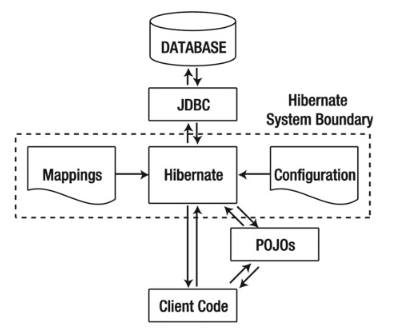
\includegraphics[width=.5\linewidth]{images/hibernateinjava}
	\caption{The role of Hibernate in a Java  application}
	\label{fig:roleofhibernate}
\end{figure}

With the advent of the World Wide Web, the demand for databases has increased. Though they may not know it, the customers of online bookshops and newspapers are using databases. Somewhere in the guts of the application, a database is being queried and a response is offered.[\cite{2}]
\newline

Hibernate is a library that simplifies the use of relational databases in Java applications by presenting relational data as simple Java objects, accessed through a session manager, therefore earning the description of being an “Object/Relational Mapper,” or ORM. It provides two kinds of programmatic interfaces: a “native Hibernate” interface and the Java EE-standard Java Persistence API.[\cite{2}]
\newline


The database is postgreSQL[\footnote{\href{https://www.postgresql.org/}{\texttt{https://www.postgresql.org/}}}]. I chose postgreSQL because has JSON support and I know in the future I will switch to a schema-less for storing the activity of a patient and was also free in the Heroku instance.

\subsubsection*{Database management systems}
Different database management systems support diverse application scenarios, use cases, and requirements. Database management systems have a long history. First we will quickly take a look at the recent history, and then explore the market-dominant database management system categories.[\cite{2}]
\newline

\subsubsection*{A brief history}
Broadly, the term database can be used to present a collection of things. Moreover, this term brings to mind many other terms including data, information, data structure, and management. A database can be defined as a collection or a repository of data, which has a certain structure, managed by a database management system(DBMS). Data can be structured as tabular data, semi-structured as XML documents, or unstructured data that does not fit a predefined data model.[\cite{14}]
\newline

In early days, databases were mainly aimed at supporting business applications; this led us to the well-defined relational algebra and relational database systems. With the introduction of object-oriented languages, new paradigms of database management systems appeared such as object-relational databases and object-oriented databases. Also, many businesses as well as scientific applications use arrays, images, and spatial data; thus, new models such as raster, map, and array algebra are supported. Graph databases are used to support graph queries such as the shortest path from one node to another along with supporting traversal queries easily.[\cite{14}]
\newline

With the advent of web applications such as social portals, it is now necessary to support a huge number of requests in a distributed manner. This has led to another new paradigm of databases called NoSQL (Not Only SQL) which has different requirements such as performance over fault tolerance and horizontal scaling capabilities.[\cite{14}]
\newline

In general, the timeline of database evolution was greatly affected by many factors such as:
\begin{itemize}
	\item Functional requirements: The nature of the applications using a DBMS has led to the development of extensions on top of relational databases such as PostGIS (for spatial data) or even dedicated DBMS such as SCI-DB (for scientific data analytics).
	\item Nonfunctional requirements: The success of object-oriented programming languages has created new trends such as object-oriented databases. Object relational database management systems have appeared to bridge the gap between relational databases and the object-oriented programming languages. Data explosion and the necessity to handle terabytes of data on commodity hardware have led to columnar databases, which can easily scale up horizontally.
\end{itemize}

\subsubsection*{Database categories}
Many database models have appeared and vanished such as the network model and hierarchal model. The predominant categories now in the market are relational, object-relational databases, and NoSQL databases. One should not think of NoSQL and SQL databases as rivals; they are complementary to each other. By utilizing different database systems, one can overcome many limitations, and get the best of different technologies.[\cite{14}]

\subsubsection*{The NoSQL databases}
The NoSQL databases are affected by the CAP theorem, also known as Brewer's theorem. In 2002, S. Gilbert and N. Lynch published a formal proof of the CAP theorem in their article: "Brewer's conjecture and the feasibility of consistent, available, partition-tolerant web services". In 2009, the NoSQL movement began. Currently, there are over 150 NoSQL databases (nosql-database.org).[\cite{14}]

\subsubsection*{The CAP theorem}
The CAP theorem states that it is impossible for a distributed computing system to simultaneously provide all three of the following guarantees:
\begin{itemize}
	\item Consistency: All clients see (immediately) the latest data even in the case of updates.
	\item Availability: All clients can find a replica of some data even in the case of a node failure. That means even if some part of the system goes down, the clients can still access the data.
	\item Partition tolerance: The system continues to work regardless of arbitrary message loss or failure of part of the system.
\end{itemize}

The choice of which feature to discard determines the nature of the system. For example, one could sacrifice consistency to get a scalable, simple, and high-performance database management system.
\newline

Often, the main difference between a relational database and a NoSQL database is consistency. A relational database enforces ACID. ACID is the acronym for the following properties: Atomicity, Consistency, Isolation, and Durability. In contrast, many NoSQL databases adopt the basically available soft-state, eventual-consistency (BASE) model.[\cite{14}]

\subsubsection*{NoSQL motivation}
A NoSQL database provides a means for data storage, manipulation, and retrieval for non-relational data. The NoSQL databases are distributed, open source and horizontally scalable. NoSQL often adopts the BASE model, which prizes availability over consistency, and informally guarantees that if no new updates are made on a data item, eventually all access to that data item will return the latest version of that data item. The advantages of this approach include the following:
\begin{itemize}
	\item Simplicity of design
	\item Horizontal scaling and easy replication
	\item Schema free
	\item Huge amount of data support
\end{itemize}

\subsubsection*{PostgreSQL}
PostgreSQL (pronounced Post-Gres-Q-L) or postgres is an open source object relational database management system. It emphasizes extensibility, creativity, as well as compatibility. It competes with the major relational database vendors such as Oracle, MySQL, SQL servers, and others. It is used by different sectors including government agencies and the public and private sectors. It is a cross-platform DBMS, and runs on most modern operating systems including Windows, MAC, and Linux flavors. It conforms to SQL, and is ACID compliant.[\cite{14}]

\subsubsection*{PostgreSQL history}
The name PostgreSQL is derived from post-ingres database. PostgreSQL history could be summarized as follows:
\begin{itemize}
	\item 1977-1985, the Ingres project: Michael Stonebraker created an RDBMS based on the formal relational model.
	\item 1986-1994, postgres: Michael Stonebraker created postgres in order to support complex data types and the object relational model.
	\item 1995, Postgres95: Andrew Yu and Jolly Chen changed the postgres POSTQUEL query language with an extended subset of SQL
	\item 1996, PostgreSQL: Several developers dedicated a lot of labor and time to stabilize postgres95. The first open source version was released on January 29, 1997. With the introduction of new features, enhancements, and due to it being an open source project, the postgres95 name was changed to PostgreSQL.
\end{itemize}


\paragraph{PostgreSQL} provides many features that attract developers, administrators, architects, and companies.
PostgreSQL is a free open source software (OSS). It is released under the PostgreSQL license, which is similar to the BSD and MIT licenses. The PostgreSQL license is highly permissive, and PostgreSQL is not subject to monopoly and acquisition. This gives the company the following advantages:
\begin{itemize}
	\item No associated licensing cost to PostgreSQL.
	\item Unlimited number of deployments of PostgreSQL.
	\item More profitable business model.
	\item PostgreSQL is SQL standards compliant; thus, finding professional developers is not very difficult. PostgreSQL is easy to learn, and porting code from one database vendor to PostgreSQL is cost efficient. Also, the PostgreSQL administrative tasks are easy to automate, thus reducing the staffing cost significantly.
	\item PostgreSQL is cross-platform, and it has drivers for all modern programming languages; so, there is no need to change the company policy regarding the software stack in order to use PostgreSQL.
	\item PostgreSQL is scalable, and it gives high performance.
	\item PostgreSQL is very reliable; it rarely crashes. Also, PostgreSQL is ACID compliant, which means that it can tolerate some hardware failure. In addition to that, it can be configured and installed as a cluster to ensure \textbf{high availability (HA)}.
\end{itemize}


\paragraph{PostgreSQL} is very attractive for developers, administrators, and architects. It has rich features that enable developers to perform tasks in an agile way. The following are some of the features that are attractive to developer:
\begin{itemize}
	\item A new release almost every year; there have been 23 major releases until now, starting from Postgres95.
	\item Very good documentation and an active community enables developers to find and solve problems quickly. The PostgreSQL manual is over 2,500 pages.
	\item A rich extension repository enables developers to focus on business logic. Also, it enables developers to meet requirement changes easily.
	\item The source code is available free of charge. It can be customized and extended without huge effort.
	\item Rich clients and administrative tools enable developers to perform routine tasks such as describing database objects, exporting and importing data, and dumping and restoring \item databases very quickly.
	\item Database administration tasks do not require a lot of time, and can be automated.
	\item PostgreSQL can be integrated easily with other database management systems giving the software architecture a good flexibility for implementing software designs.
\end{itemize}

\paragraph{Success stories}
PostgreSQL is used in many application domains including communication, medical, geographical, and e-commerce applications. Many companies provide consultation as well as commercial services, such as migrating proprietary RDBMS to PostgreSQL in order to cut off the licensing costs. These companies often influence and enhance PostgreSQL by developing and submitting new features.
\newline

The following are a few companies that have used PostgreSQL:
\begin{itemize}
	\item Skype uses PostgreSQL to store user chats and activities. Skype has also affected PostgreSQL by developing many tools called Skytools.
	\item Instagram is a social networking service that enables its user to share pictures and photos. Instagram has more than 100 million active users.
	\item The American chemical society (ACS) uses PostgreSQL to store more than one terabyte of data for the journal archive.
\end{itemize}
In addition to the companies mentioned in the preceding list, PostgreSQL is used by HP, WMware, and Heroku. PostgreSQL is used by many scientific communities and organizations, such as NASA, due to its extensibility and rich data types.

\subsection{Frontend}
The frontend is a web application, is based on the classic web technologies: HTML5[\footnote{\href{https://en.wikipedia.org/wiki/HTML5}{\texttt{https://en.wikipedia.org/wiki/HTML5}}}], CSS3[\footnote{\href{https://en.wikipedia.org/wiki/Cascading\_Style\_Sheets}{\texttt{https://en.wikipedia.org/wiki/Cascading\_Style\_Sheets}}}] and JavaScript[\footnote{\href{https://en.wikipedia.org/wiki/JavaScript}{\texttt{https://en.wikipedia.org/wiki/JavaScript}}}]. On top of that I used the Bootstrap[\footnote{\href{https://getbootstrap.com/}{\texttt{https://getbootstrap.com/}}}] framework for having a responsive web page and for the routing and consuming the backend RESTapi I decided to use AngularJs[\footnote{\href{https://angularjs.org/}{\texttt{https://angularjs.org/}}}].


\subsubsection*{HTML (HyperText Markup Language)}
HyperText Markup Language, commonly referred to as HTML, is the standard markup language used to create web pages. It is written in the form of HTML elements consisting of tags enclosed in angle brackets (like <html>). HTML tags most commonly come in pairs like <h1> and </h1>, although some represent empty elements and so are unpaired, for example <img>. The first tag in such a pair is the start tag, and the second is the end tag (they are also called opening tags and closing tags).
\newline

Web browsers can read HTML files and render them into visible or audible web pages. Browsers do not display the HTML tags and scripts, but use them to interpret the content of the page. HTML describes the structure of a website semantically along with cues for presentation, making it a markup language, rather than a programming language.
\newline
\begin{figure}[h]
	\centering
	
\includegraphics[width=0.4\linewidth]{images/HTML5_Logo_512}
	\captionof{figure}{HTML 5}
	\label{fig:html-logo}
\end{figure}
HTML elements form the building blocks of all websites. HTML allows images and objects to be embedded and can be used to create interactive forms. It provides a means to create structured documents by denoting structural semantics for text such as headings, paragraphs, lists, links, quotes and other items. It can embed scripts written in languages such as JavaScript which affect the behavior of HTML web pages.
Web browsers can also refer to Cascading Style Sheets (CSS) to define the look and layout of text and other material. The World Wide Web Consortium (W3C), maintainer of both the HTML and the CSS standards, has encouraged the use of CSS over explicit presentational HTML since 1999.[\cite{7}]

\subsubsection*{JavaScript}
JavaScript is the programming language of the Web. The overwhelming majority of
modern websites use JavaScript, and all modern web browsers on desktops, game
consoles, tablets, and smart phones—include JavaScript interpreters, making JavaScript
the most ubiquitous programming language in history. JavaScript is part of the
triad of technologies that all Web developers must learn: HTML to specify the content
of web pages, CSS to specify the presentation of web pages, and JavaScript to specify
the behavior of web pages. This book will help you master the language.
If you are already familiar with other programming languages, it may help you to know
that JavaScript is a high-level, dynamic, untyped interpreted programming language
that is well-suited to object-oriented and functional programming styles. JavaScript
derives its syntax from Java, its first-class functions from Scheme, and its prototypebased
inheritance from Self. But you do not need to know any of those languages, or
be familiar with those terms, to use this book and learn JavaScript.[\cite{12}]
\newline
\begin{figure}[h]
	\centering
	
\includegraphics[width=0.4\linewidth]{images/js}
	\captionof{figure}{JavaScript}
	\label{fig:js-logo}
\end{figure}
The name “JavaScript” is actually somewhat misleading. Except for a superficial syntactic
resemblance, JavaScript is completely different from the Java programming language.
And JavaScript has long since outgrown its scripting-language roots to become
a robust and efficient general-purpose language. The latest version of the language (see
the sidebar) defines new features for serious large-scale software development.[\cite{12}]  

\subsubsection*{CSS (Cascading Style Sheets)}
Cascading Style Sheets (CSS) is a style sheet language used for describing the look and formatting of a document written in a markup language. While most often used to change the style of web pages and user interfaces written in HTML and XHTML, the language can be applied to any kind of XML document, including plain XML, SVG and XUL. Along with HTML and JavaScript, CSS is a cornerstone technology used by most websites to create visually engaging webpages, user interfaces for web applications, and user interfaces for many mobile applications.[\cite{7}]
\newline

CSS is designed primarily to enable the separation of document content from document presentation, including elements such as the layout, colors, and fonts. This separation can improve content accessibility, provide more flexibility and control in the specification of presentation characteristics, enable multiple HTML pages to share formatting by specifying the relevant CSS in a separate .css file, and reduce complexity and repetition in the structural content, such as semantically insignificant tables that were widely used to format pages before consistent CSS rendering was available in all major browsers. CSS makes it possible to separate presentation instructions from the HTML content in a separate file or style section of the HTML file. For each matching HTML element, it provides a list of formatting instructions. For example, a CSS rule might specify that "all heading 1 elements should be bold," leaving pure semantic HTML markup that asserts "this text is a level 1 heading" without formatting code such as a <bold> tag indicating how such text should be displayed.[\cite{7}]
\newline
\begin{figure}[h]
		\centering
		
\includegraphics[width=0.4\linewidth]{images/css3_icon}
		\captionof{figure}{CSS 3}
		\label{fig:css-logo}
\end{figure}
This separation of formatting and content makes it possible to present the same markup page in different styles for different rendering methods, such as on-screen, in print, by voice (when read out by a speech-based browser or screen reader) and on Braille-based, tactile devices. It can also be used to display the web page differently depending on the screen size or device on which it is being viewed. While the author of a web page typically links to a CSS file within the markup file, readers can specify a different style sheet, such as a CSS file stored on their own computer, to override the one the author has specified. If the author or the reader did not link the document to a style sheet, the default style of the browser will be applied. Another advantage of CSS is that aesthetic changes to the graphic design of a document (or hundreds of documents) can be applied quickly and easily, by editing a few lines in one file, rather than by a laborious (and thus expensive) process of crawling over every document line by line, changing markup.[\cite{7}]
\newline

The CSS specification describes a priority scheme to determine which style rules apply if more than one rule matches against a particular element. In this so-called cascade, priorities or weights are calculated and assigned to rules, so that the results are predictable.
The CSS specifications are maintained by the World Wide Web Consortium (W3C). Internet media type (MIME type) text/css is registered for use with CSS by RFC 2318 (March 1998). The W3C operates a free CSS validation service for CSS documents.[\cite{7}]

\subsubsection*{Less (stylesheet language)}
Less (sometimes stylized as LESS) is a dynamic stylesheet language that can be compiled into Cascading Style Sheets (CSS), or can run on the client-side and server-side. Designed by Alexis Sellier, Less is influenced by Sass and has influenced the newer "SCSS" syntax of Sass, which adapted its CSS-like block formatting syntax. Less is open-source. Its first version was written in Ruby, however in the later versions, use of Ruby has been deprecated and replaced by JavaScript. The indented syntax of Less is a nested metalanguage, as valid CSS is valid Less code with the same semantics. Less provides the following mechanisms: variables, nesting, mixins, operators and functions; the main difference between Less and other CSS precompilers being that Less allows real-time compilation via less.js by the browser.[\cite{7}]

\subsubsection*{AngularJs}
There was a time many internet years ago when any kind of logic within a web pagehad to be sent to the server for processing and then re-rendered as an entirely newweb page. This “call and refresh” arrangement made for a disjointed user experi-ence, which was only exacerbated when network latency was especially high.[\cite{1}]  
\newline

The  entire  paradigm  was  upended  with  the  introduction  of  XMLHttpRequestand the ability to make asynchronous calls to the server without actually having torefresh  the  page. This  made  for  a  much  more  coherent  user  experience  becausethe user could perform a task that required a remote call and still interact with theapplication as the call was being made and processed. This is where the first wave ofJavaScript frameworks landed and managed to prove that working with JavaScript could be done in a mostly sane way and no one was going to lose life or limb.[\cite{1}]  
\newline
\begin{figure}[h]
		\centering
		
\includegraphics[width=0.7\linewidth]{images/angular}
		\captionof{figure}{AngularJs}
		\label{fig:angular-logo}
\end{figure}
Most  people  would  agree  that  jQuery  won  that  round,  partially  because  jQuerydid such a good job of abstracting away all of the insanity surrounding browser varia-tions,  and  allowed  developers  to  use  a  single,  simplified  API  to  build  websites.  Thenext frontier was to make websites behave and operate as if they were actual applica-tions; this ushered in an entirely new set of challenges. For instance, jQuery has donean  exceptional  job  of  providing  tools  to  manipulate  the  DOM,  but  it  offers  no  realguidance on how to organize your code into an application structure. We’ve all heardhorror  stories  of  how  a  jQuery  “application”  ballooned  out  into  a  monstrosity  thatcould barely be maintained, much less extended.[\cite{1}]  
\newline

This desperate need to write large, maintainable JavaScript applications has givenbirth to a JavaScript framework renaissance. In the last couple of years, a slew of frame-works has burst onto the scene, with many of them quietly fading off into oblivion. Buta few frameworks have proven themselves to be solid options for writing large-scale webapplications that can be maintained, extended, and tested. One of the most popular, ifnot the most popular, frameworks to emerge is AngularJS from Google.[\cite{1}]  
\newline

AngularJS is an open-source web application framework that offers quite a bit to adeveloper  through  a  stable  code  base,  vibrant  community,  and  rich  ecosystem.[\cite{1}]  


\subsubsection*{Bootstrap}
\begin{figure}[h]
	\centering
	
\includegraphics[width=.5\linewidth]{images/bootstrap}
	\captionof{figure}{Bootstrap}
	\label{fig:bootstrap-logo}
\end{figure}
Bootstrap, originally named Twitter Blueprint, was developed by Mark Otto and Jacob Thornton at Twitter as a framework to encourage consistency across internal tools. Before Bootstrap, various libraries were used for interface development, which led to inconsistencies and a high maintenance burden. According to Twitter developer Mark Otto:
\newline

\textit{"A super small group of developers and I got together to design and build a new internal tool and saw an opportunity to do something more. Through that process, we saw ourselves build something much more substantial than another internal tool. Months later, we ended up with an early version of Bootstrap as a way to document and share common design patterns and assets within the company."}
\newline

After a few months of development by a small group, many developers at Twitter began to contribute to the project as a part of Hack Week, a hackathon-style week for the Twitter development team. It was renamed from Twitter Blueprint to Bootstrap, and released as an open source project on August 19, 2011. It has continued to be maintained by Mark Otto, Jacob Thornton, and a small group of core developers, as well as a large community of contributors.
\newline

On January 31, 2012, Bootstrap 2 was released, which added a twelve-column responsive grid layout system, inbuilt support for Glyphicons, several new components, as well as changes to many of the existing components.
\newline

On August 19, 2013, Bootstrap 3 was released, which redesigned components to use flat design, and a mobile first approach.
\newline

On October 29, 2014, Mark Otto announced that Bootstrap 4 was in development. The first alpha version of Bootstrap 4 was released on August 19, 2015.[\cite{1}]  
%\begin{figure}[h]
%	\centering
%	\begin{minipage}{\textwidth}
%		\centering
%		
\includegraphics[width=0.7\linewidth]{images/angular}
%		\captionof{figure}{AngularJs}
%		\label{fig:angular-logo}
%	\end{minipage}
%	\begin{minipage}{.5\textwidth}
%		\centering
%		
\includegraphics[width=0.4\linewidth]{images/HTML5_Logo_512}
%		\captionof{figure}{HTML 5}
%		\label{fig:html-logo}
%	\end{minipage}%
%	\begin{minipage}{.5\textwidth}
%		\centering
%		
\includegraphics[width=0.4\linewidth]{images/css3_icon}
%		\captionof{figure}{CSS 3}
%		\label{fig:css-logo}
%	\end{minipage}
%
%	\begin{minipage}{.5\textwidth}
%		\centering
%		
\includegraphics[width=0.4\linewidth]{images/js}
%		\captionof{figure}{JavaScript}
%		\label{fig:js-logo}
%	\end{minipage}%
%	\begin{minipage}{.5\textwidth}
%		\centering
%		
\includegraphics[width=.5\linewidth]{images/bootstrap}
%		\captionof{figure}{Bootstrap}
%		\label{fig:bootstrap-logo}
%	\end{minipage}
%	\begin{minipage}{.5\textwidth}
%		\centering
%		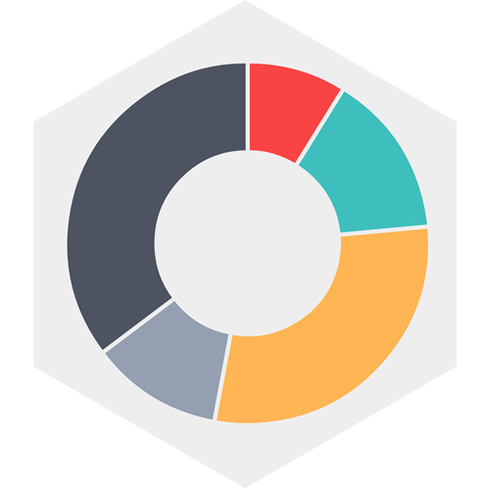
\includegraphics[width=.5\linewidth]{images/chartjs}
%		\captionof{figure}{Chartjs}
%		\label{fig:chartjs-logo}
%    \end{minipage}
%\end{figure}

%\begin{figure}[h]
%	\centering
%	\begin{minipage}{.5\textwidth}
%		\centering
%		
\includegraphics[width=.4\linewidth]{images/npm}
%		\captionof{figure}{npm}
%		\label{fig:npm-logo}
%	\end{minipage}%
%	\begin{minipage}{.5\textwidth}
%		\centering
%		
\includegraphics[width=.4\linewidth]{images/bower}
%		\captionof{figure}{Bower}
%		\label{fig:bower-logo}
%	\end{minipage}
%
%	\begin{minipage}{.5\textwidth}
%		\centering
%		
\includegraphics[width=.5\linewidth]{images/grunt}
%		\captionof{figure}{GruntJs}
%		\label{fig:grunt-logo}
%	\end{minipage}
%\end{figure}

\subsection{Daemon}
The daemon is a python application and can be run only on a linux machine.
Prerequisites
\begin{itemize}
	\item python 3.4+
    \item bluez 5.43+
	\item glib 2
	\item python pip
\end{itemize}
Then you need to clone the repository and configure the MAC address for the smartbands in config/db.json
\begin{lstlisting}[language=Bash]
git clone https://lupu60@bitbucket.org/gnp_team/client-python.git
python3 ClientMain
\end{lstlisting}
Python is a widely used high-level programming language for general-purpose programming, created by Guido van Rossum and first released in 1991. An interpreted language, Python has a design philosophy which emphasizes code readability (notably using whitespace indentation to delimit code blocks rather than curly brackets or keywords), and a syntax which allows programmers to express concepts in fewer lines of code than might be used in languages such as C++ or Java.The language provides constructs intended to enable writing clear programs on both a small and large scale.
\newline

Python features a dynamic type system and automatic memory management and supports multiple programming paradigms, including object-oriented, imperative, functional programming, and procedural styles. It has a large and comprehensive standard library.
\newline

Python interpreters are available for many operating systems, allowing Python code to run on a wide variety of systems. CPython, the reference implementation of Python, is open source software and has a community-based development model, as do nearly all of its variant implementations. CPython is managed by the non-profit Python Software Foundation.[\cite{6}]  
\begin{lstlisting}[language=Bash]
{
	"configuration": {
		"1": {
			"deviceId": "C8:0F:10:33:A8:3C",
			"userInfo": {
				"alias": "Jan",
				"gender": 1,
				"weight": 78,
				"age": 29,
				"height": 180
			}
		}
	}
}
\end{lstlisting}


\section{Toolchain}
In software, a toolchain is a set of programming tools that are used to perform a complex software development task or to create a software product, which is typically another computer program or a set of related programs. In general, the tools forming a toolchain are executed consecutively so the output or resulting environment state of each tool becomes the input or starting environment for the next one, but the term is also used when referring to a set of related tools that are not necessarily executed consecutively.
\newline

First of all the codebase is hosted on bitbucket in a git repository[\footnote{\href{https://lupu60@bitbucket.org/gnp\_team/backend.git}{\texttt{https://lupu60@bitbucket.org/gnp\_team/backend.git}}}], I choose bitbucket because it`s free to host private repository and also for the new feature bitbucket pipelines witch is a continuous delivery system(Figure \ref{fig:piplines}). 
\newline

Continuous delivery (CD) is a software engineering approach in which teams produce software in short cycles, ensuring that the software can be reliably released at any time. It aims at building, testing, and releasing software faster and more frequently. The approach helps reduce the cost, time, and risk of delivering changes by allowing for more incremental updates to applications in production. A straightforward and repeatable deployment process is important for continuous delivery.
\newline

At a code change on the repository the pipeline will compile my code and deploy to Heroku. In the repository I used the git flow model[\footnote{\href{http://nvie.com/posts/a-successful-git-branching-model/}{\texttt{http://nvie.com/posts/a-successful-git-branching-model/}}}] for the branching strategy.
\begin{figure}[h]
	\centering
	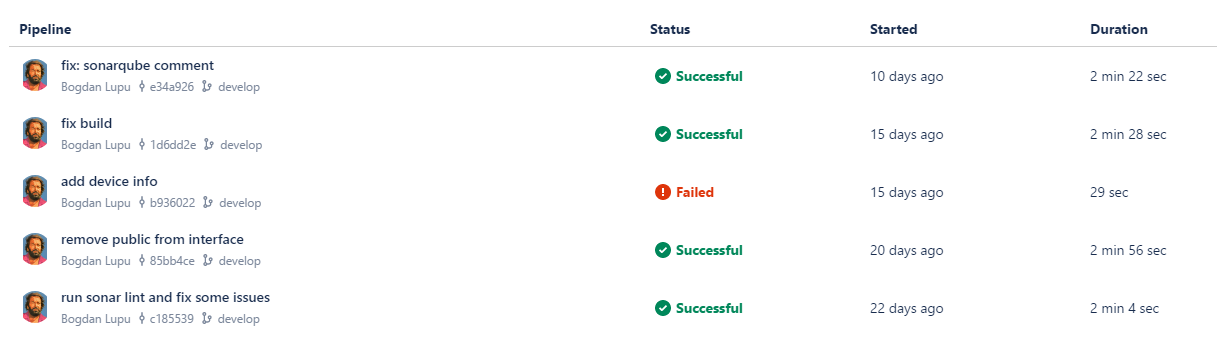
\includegraphics[width=\linewidth]{images/pipelines}
	\caption{Bitbucket Pipelines Dashboard}
	\label{fig:piplines}
\end{figure}

The IoT healthcare  has 2 cloud instance a live/production[\footnote{\href{https://iothealthcare.herokuapp.com/}{\texttt{https://iothealthcare.herokuapp.com/}}}] and a prelive/integration [\footnote{\href{https://intiothealthcare.herokuapp.com/}{\texttt{https://intiothealthcare.herokuapp.com/}}}]. This strategy I used is really usefully because I can separate the codebase and not allowing bugs to be on the production. So in the first step I coded local and tested then I push my code to the develop branch form the repository and the bitbucket pipeline will deploy the develop branch on integration and master branch on production, all of this is made it by a bash script. So after I test my code also on the Heroku enviroment I can merge my code from develop to master.
For the code quality I have a sonarQube(Figure \ref{fig:sonar}) instance with docker on my localhost and I run it from time to time. 
\newline
\begin{figure}[h]
	\centering
	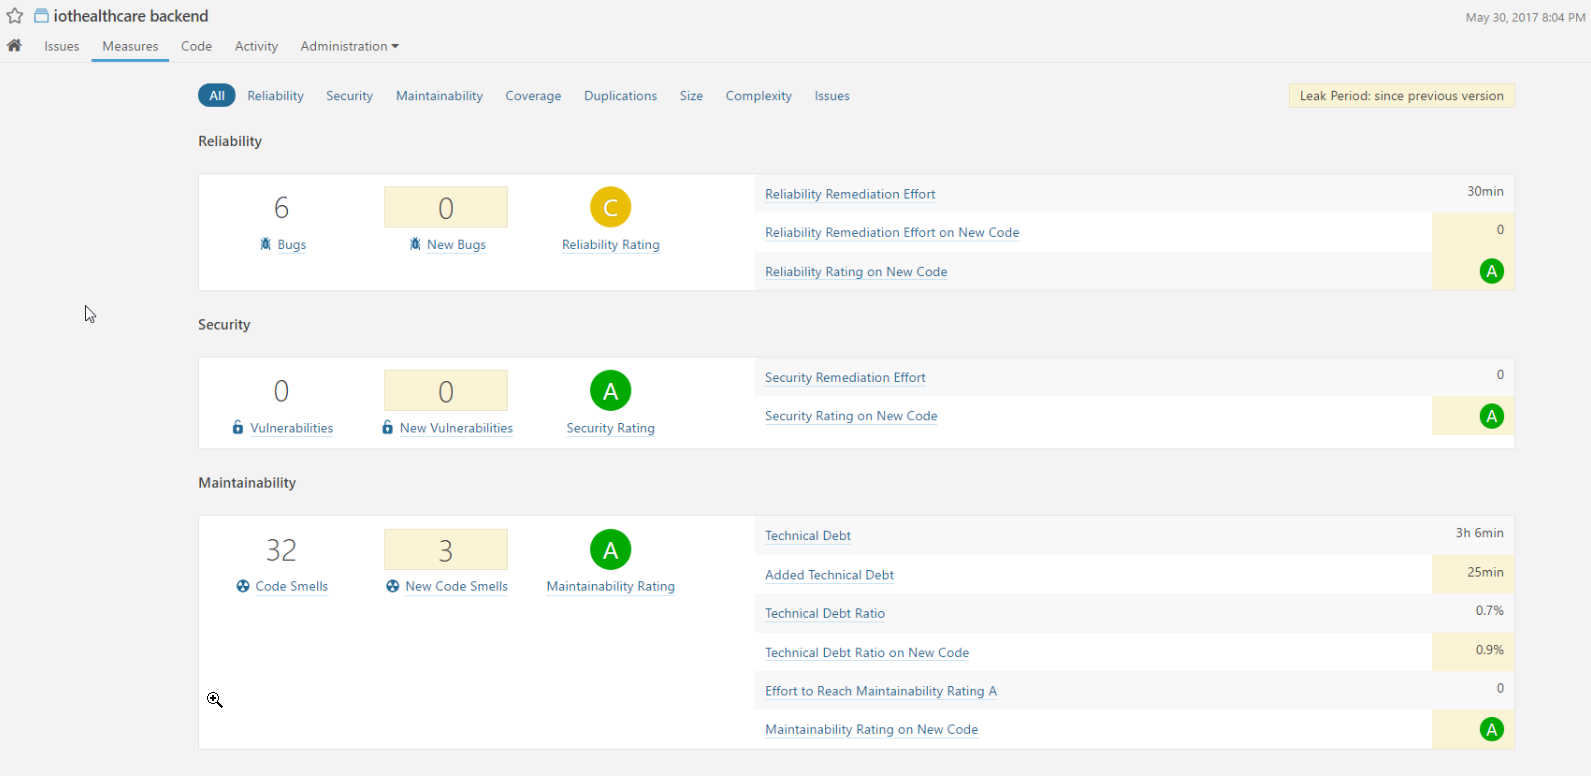
\includegraphics[width=\linewidth]{images/sonarqube}
	\caption{IoT Healthcare: sonarQube build}
	\label{fig:sonar}
\end{figure}
SonarQube is an open source platform for continuous inspection of code quality.
\newline
In the context of software engineering, software quality refers to two related but distinct notions that exist wherever quality is defined in a business context:
\begin{itemize}
	\item Software functional quality reflects how well it complies with or conforms to a given design, based on functional requirements or specifications. That attribute can also be described as the fitness for purpose of a piece of software or how it compares to competitors in the marketplace as a worthwhile product. It is the degree to which the correct software was produced.
	\item Software structural quality refers to how it meets non-functional requirements that support the delivery of the functional requirements, such as robustness or maintainability. It has a lot more to do with the degree to which the software works as needed.
\end{itemize}
Many aspects of structural quality can be evaluated only statically through the analysis of the software inner structure, its source code, at the unit level, the technology level and the system level, which is in effect how its architecture adheres to sound principles of software architecture outlined in a paper on the topic by OMG. But some structural qualities, such as usability, can be assessed only dynamically (users or others acting in their behalf interact with the software or, at least, some prototype or partial implementation; even the interaction with a mock version made in cardboard represents a dynamic test because such version can be considered a prototype). Other aspects, such as reliability, might involve not only the software but also the underlying hardware, therefore, it can be assessed both statically and dynamically (stress test).
Functional quality is typically assessed dynamically but it is also possible to use static tests (such as software reviews).
Historically, the structure, classification and terminology of attributes and metrics applicable to software quality management have been derived or extracted from the ISO 9126-3 and the subsequent ISO 25000:2005[3] quality model, also known as SQuaRE.[4] Based on these models, the Consortium for IT Software Quality (CISQ) has defined five major desirable structural characteristics needed for a piece of software to provide business value: Reliability, Efficiency, Security, Maintainability and (adequate) Size.[\footnote{\href{https://de.wikipedia.org/wiki/Statische\_Code-Analyse}{\texttt{https://de.wikipedia.org/wiki/Statische\_Code-Analyse}}}]
\newline


Software quality measurement quantifies to what extent a software or system rates along each of these five dimensions. An aggregated measure of software quality can be computed through a qualitative or a quantitative scoring scheme or a mix of both and then a weighting system reflecting the priorities. This view of software quality being positioned on a linear continuum is supplemented by the analysis of "critical programming errors" that under specific circumstances can lead to catastrophic outages or performance degradations that make a given system unsuitable for use regardless of rating based on aggregated measurements. Such programming errors found at the system level represent up to 90\% of production issues, whilst at the unit-level, even if far more numerous, programming errors account for less than 10\% of production issues. As a consequence, code quality without the context of the whole system, as W. Edwards Deming described it, has limited value.[\footnote{\href{https://de.wikipedia.org/wiki/Statische\_Code-Analyse}{\texttt{https://de.wikipedia.org/wiki/Statische\_Code-Analyse}}}]
\newline
 
To view, explore, analyze, and communicate software quality measurements, concepts and techniques of information visualization provide visual, interactive means useful, in particular, if several software quality measures have to be related to each other or to components of a software or system. For example, software maps represent a specialized approach that "can express and combine information about software development, software quality, and system dynamics".
\newline

Now I will present who to run the app and the tools need it.

Necessary installed programs.
\begin{itemize}
	\item Java
	\item nodejs
	\item docker
	\item git
	\item postgreSql (is possible to use a docker image for postgres also)
\end{itemize}
\vspace{5mm}

After you have installed all this programs. First thing we need to do is to clone the repository. So open a command prompt and type the following commands.
\begin{lstlisting}[language=Bash]
git clone https://lupu60@bitbucket.org/gnp_team/backend.git ioth
\end{lstlisting}
\vspace{5mm}

Then configure the database connections properties to connect to the local database in the application.properties file which is located in /src/main/resource.
\begin{lstlisting}[language=Bash]
#localhost POSTGRESQL
spring.datasource.url= jdbc:postgresql://localhost:5432/ioth
spring.datasource.username=postgres
spring.datasource.password=4NzgY09ZdnhZbVir3fUk
\end{lstlisting}
\vspace{5mm}

Now we just need to build the app and start so in the cmd:
\begin{lstlisting}[language=Bash]
cd ioth
npm install -g grunt-cli
npm install -g bower
npm install
gradlew clean build run
\end{lstlisting}
\vspace{5mm}

Access http://localhost:8080/ and the login credentials are user/user. For running the sonarQube you need to install the sonarDocker container and then run the gradlew script but first generate a personal toke form the sonar web interface.
\begin{lstlisting}[language=Bash]
cd ioth
gradlew clean build sonarqube -Dsonar.host.url=http://localhost:<port>
-Dsonar.token=<token>
\end{lstlisting}
\vspace{5mm}

For deploying the app on Heroku after some changes just push the code the default configuration is for the integration, for production open a pull request or merge the develop to master and push.
\begin{lstlisting}[language=Bash]
git checkout master
git pull -r
git merge develop
git push
\end{lstlisting}

For testing the restApi I used postman the postman colletion are avaible in the repostiory in the folder postmanconf.
\begin{figure}[h]
	\centering
	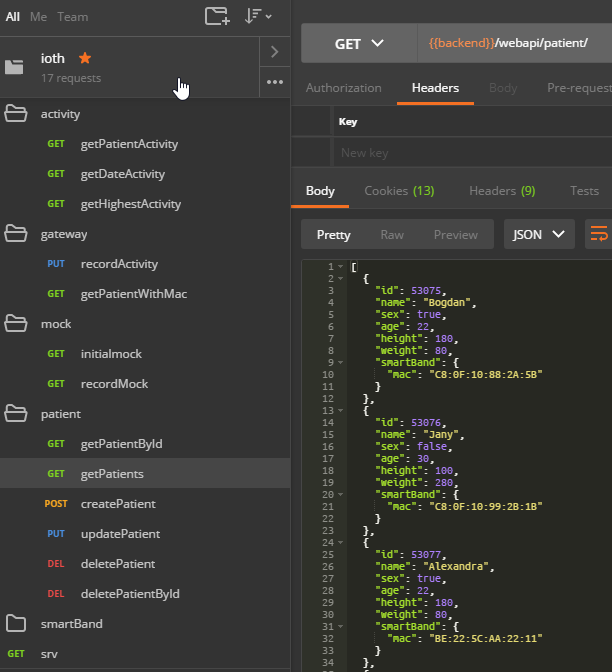
\includegraphics[width=0.6\linewidth]{images/postman}
	\caption{Postman Dashboard}
	\label{fig:postman}
\end{figure}

\section{Tools Used for Development Process}
\subsection{Heroku}
Heroku[\footnote{\href{https://www.heroku.com/home}{\texttt{https://www.heroku.com/home}}}] is a cloud platform as a service (PaaS) supporting several programming languages that is used as a web application deployment model. Heroku, one of the first cloud platforms, has been in development since June 2007, when it supported only the Ruby programming language, but now supports Java, Node.js, Scala, Clojure, Python, PHP, and Go. For this reason, Heroku is said to be a polyglot platform as it lets the developer build, run and scale applications in a similar manner across all the languages. Heroku was acquired by Salesforce.com in 2010 for \$212 million.
\newline
\begin{figure}[h!]
	\centering
	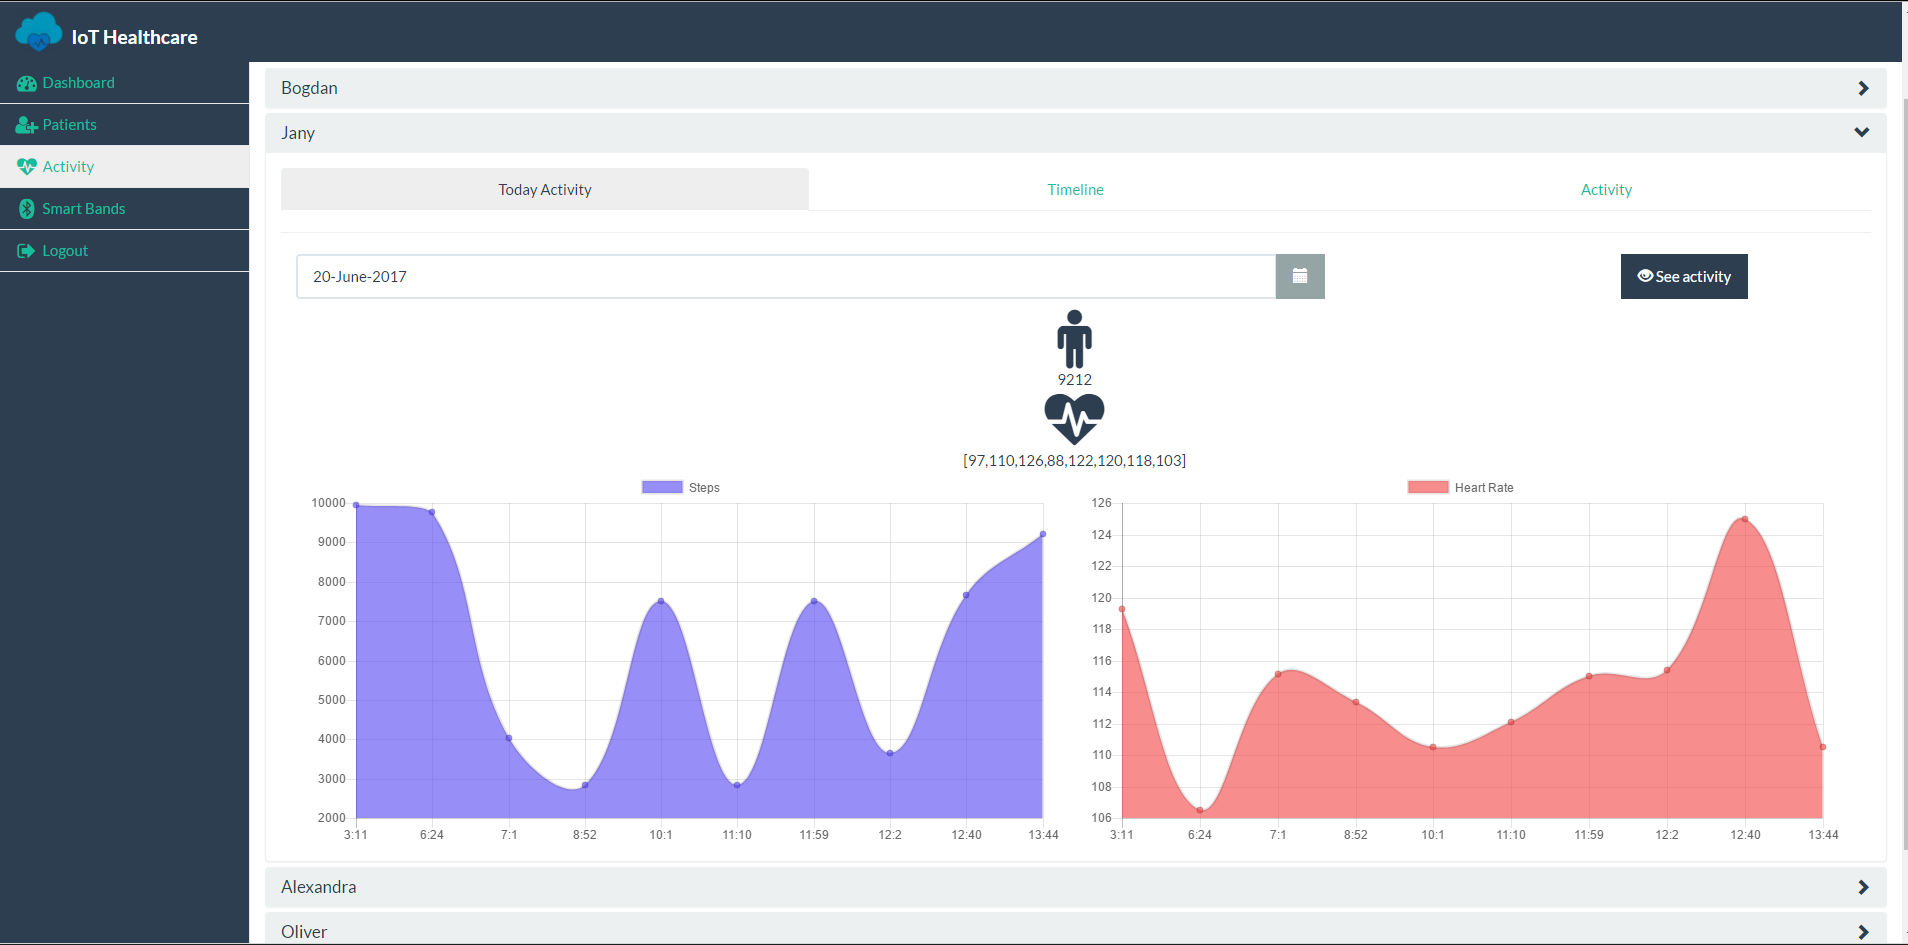
\includegraphics[width=1\textwidth]{./images/iothheroku}
	\rule{1\textwidth}{1pt}
	\caption{IoT Healthcare running on herokucloud}
	\label{fig:iothoh}
\end{figure}
The notion of service is central to cloud computing. It is so central that a capability offered through the cloud gains differentiation by appending “-as-a-service” to a legacy product offering, thus presumably increasing its perceived value. Therefore, we get the terms software-as-a-service (SaaS), platform-as-a-service (PaaS) and infrastructure-as-a-service (IaaS); and yet there is very little in the cloud literature that clarifies what service, and services, actually are. To some, the concept of service survives as a primitive notion. Within a body of knowledge such as cloud computing, a primitive notion is an undefined concept that defies definition in terms of previously defined concepts. As a result, the IT practitioner informally applies meaning to a concept through experience or intuition. For instance, the Rackspace and National Institute of Standards and Technology publications focus on cloud-based services, but the concept itself is not clearly defined. The presentations contrast cloud services characteristics with those of customer-owned non-cloud product capabilities. The practitioner considers the features, advantages, and benefits in terms of the existing product solution.
\newline

From the traditional product perspective, services are add-on extensions of a physical product, intangible products, or services solutions that are developed and marketed as products. This services-for-a-product approach indicates a goods-dominant logic (GDL) that conceptualizes and designs services as units of output that embed and deliver value to the customer. GDL expresses as a value-in-exchange, arm's-length transaction. There is no expectation of an ongoing relationship or collaboration between the service provider and customer. This is the primitive notion that services should be defined in terms of what we know from experience, our product familiarity. Indeed, we differentiate this product view by using the plural services when a GDL perspective indicates.
\newline

The service science discipline and its service-dominant logic (SDL) provides an alternative paradigm, with service as a process that involves providers, customers and other complementary actors within a service ecosystem for the purpose of co-creating value. It emphasizes a value-in-use and value-in-context to the service network approaches to value creation. Service providers and customers benefit from the collaborative exchange of knowledge, skills, technology and other resources within the service ecosystem. The co-creation process can result in superior service design, quality, pricing, customer service, and user experiences that inform compelling value propositions and realized value for all participants. Cloud computing has opened the door for the development of SDL service innovation business models. No longer constrained by GDL thinking, the cloud, especially the multi-sided platform models disrupting e-commerce, transportation, and hospitality and big data analytics, to name a few industries, have the potential to not only redefine cloud service business models, but whole industries as well. In our view, to realize the full potential of the cloud requires an integration of service science principles with cloud computing practice. The cloud is about service and increasingly service is about the cloud.[\cite{24}]
\newline

The primary goal for this book is to apply the service innovation principles to cloud computing. This book is one of the first attempts to integrate these disciplines. The motivation for this exercise is eminently practical, especially to technologists, systems and solutions architects, as well as CIOs and business strategists. As we gain insight into technology development and integration dynamics, we can reason and engage in prediction and forecasting exercises. We understand how approaches in use by product-oriented companies do not satisfactorily apply to the service-oriented cloud. We also discover that there is a path for transformation for product-oriented organizations to operate optimally in the cloud space and therefore to attain a sustained and strategic competitive advantage. This is especially applicable to technology companies with long-term product roadmaps. These companies can servitize existing product lines as an interim step in the transition toward becoming cloud-based service enterprises. The cloud-as-a-service opens up opportunities for new revenue streams and revenue modalities, converting "lumpy" revenue that depend on big bang new product launches to a more sustained service-oriented recurrent revenue. [\cite{19}]
\newline

By employing a cloud-service framework, it is now easier to understand emerging technology progressions that seemed related, but difficult to explain and operationalize. For instance, the much-heralded progression from cloud computing to the Internet of Things (IoT) domain. This understanding allows an organization to approach the cloud and IoT under a single, unified and synergistic strategy at a fraction of the cost of developing two separate strategies. In fact, the effect of two separate efforts will be less than synergistic. The overlap of the two functions will likely result in channel conflicts, with the two organizations working against each other. For this reason, we believe that traditional, product-oriented companies cannot just look at the cloud as just a new, emerging market. These companies will need to adopt a service ethic from within, meaning adopting a service ethic from within; in the methodologies used to develop technology and in the way they conduct business processes. These organizations will suffer from the drag of the dissonance between the SDL and GDL approaches. Conversely, companies adopting an SDL approach early on will enjoy an inherent and sustained competitive advantage in the cloud market.
\newline
\subsubsection*{Software as a Service (SaaS)}
The idea of “Software as a Service” isn’t new, but the term SaaS is. SaaS simply refersto software that is provided on-demand for use. Traditionally, when someone wantedto use software they’d go to the store, pick up some disks, take them home, and installthem on a computer. With SaaS, they just use hosted software. There’s no installation, no updates, no mess. There’s no magic to it. Anyone who has used web mail of anykind has been using SaaS.
\newline

SaaS has really come into maturity over the last decade. Some modern SaaS providers do a lot of fancy work behind the scenes to make things function properly. Comparewhat engineers had to do to run web mail in the late 90s to what the team at Google does to run Gmail today.[\cite{19}]
\newline

If one of those web mail admins from the 90s were brought forward in time and toldto use Gmail, they’d be impressed for sure, but the basic workflow and usage wouldbe very familiar to them. If that same sysadmin was told to start running Gmail, he’dlikely be completely lost. That’s a common theme in cloud computing. Some aspects are so familiar, yet others are quite foreign when compared to traditional computing environments.[\cite{19}]
\subsubsection*{Infrastructure as a Service (IaaS)}
nfrastructure as a Service (IaaS) isn’t conceptually new. People have been collocatingin data centers since data centers have been around. What is different with IaaS is thetooling behind it and where the lines of responsibility get drawn. Proper IaaS providesa mechanism for people to replace all of their data center hardware needs. CommonIaaS services include:[\cite{19}]
\begin{itemize}
	\item Host provisioning
	\item Load balancing
	\item Public and private network connectivity
	\item Firewalls
	\item Storage
\end{itemize}
Additionally, all of the dependencies for these services are also provided. This includesmonitoring, power, cooling, repair, security, inventory tracking, and perhaps mostimportantly, people. Some IaaS providers even have convenient solutions to geograph-ically diversify computing resources. All of this is provided at a cost that just isn’tpossible with traditional computing. Typical rates for a host are pennies an hour.
\newline

In practical terms, this means that the time between when someone decides they needto host to when they actually log into it has been greatly reduced to a couple of minutes.Developers don’t have to put a large proposal together that includes servers, storage,network, rack space, installation, configuration, and so on. An entire proof of conceptcan be put together for the cost of a typical lunch. They don’t have to wait hours forsysadmins to provision a host. They don’t have to wait days for an order to get deliveredand installed. Instead, with IaaS, they just need a little cash and a few minutes to pickwhat host they want.

\subsubsection*{Platform as a Service (PaaS)}
Unlike IaaS and SaaS, PaaS is a much more abstract concept. Looking at cloud com-puting as an entire stack, PaaS would be in the middle of that stack. With IaaS at thebottom and SaaS at the top to interface with the end users and consumers. That’s notto imply all layers of the stack are required at once to consider yourself to be usingcloud computing.
\newline

PaaS providers offer a platform for others to use. What is being provided is part oper-ating system and part middleware. A proper PaaS provider takes care of everythingneeded to run some specific language or technology stack. Lets take a look at what itwould take to provide a Python development interface and what that means for thePaaS user.
\newline

In order for Python code to be run, developers need the Python runtime and some sortof interface to expose the Python code while it’s running. Some PaaS providers thatsupport Python do it via a WSGI2 interface. Apache, with the mod\_wsgi module, isone such way to run Python applications. Developers or PaaS providers need a WSGIscript somewhere so the code can be loaded and exposed via a web address.
\newline

To visualize this, think about Apache and Python at a public web address with somestorage on the back end and maybe a load balancer seems pretty simple to do. Don’tforget though, that there’s a whole set of dependencies in order to get to that point.Apache needs some sort of operating system to function. It needs to be configured,maintained and monitored. In cloud computing, this OS runs inside virtual machines.[\cite{19}]
\newline

This gets into the details of the IaaS layer mentioned earlier. PaaS providers may dothis themselves, or partner with an IaaS vendor to get it done. The important bit ofinformation here is to know that everything from the running Apache/WSGI interfaceall the way down to the power and cooling in a data center, is someone else’s respon-sibility. It is not the responsibility of the PaaS consumer.
\newline

\textit{Many PaaS providers are providing muti-tenant solutions. This meansthat not only is the physical hardware shared among multiple virtualmachines but the virtual machines themselves may have several differentapplications from several different customers on them.}
\newline

PaaS today focuses almost entirely on web solutions. The components an end userinteracts with are all web-based and because of this, most PaaS providers excel whenit comes to large numbers of short lived process requests. PaaS providers have less polishwhen it comes to longer running, higher resource intensive jobs that cannot be brokendown into smaller jobs. For example, a large batch processing job is likely best suitedto be placed a level down at the IaaS layer because of the more fine controls over memoryit provides. Scale out, not up, is becomming a common theme used throughout thisbook. It’s not a good or bad thing, but it’s a common architectural limitation. As PaaSmatures, expect to see more offerings beyond web services.[\cite{19}]

\subsection{Bitbucket}
Bitbucket[\footnote{\href{https://bitbucket.org/}{\texttt{https://bitbucket.org/}}}] is a web-based hosting service that is owned by Atlassian, used for source code and development projects that use either Mercurial (since launch) or Git (since October 2011) revision control systems. Bitbucket offers both commercial plans and free accounts. It offers free accounts with an unlimited number of private repositories (which can have up to five users in the case of free accounts) as of September 2010. Bitbucket integrates with other Atlassian software like Jira, HipChat, Confluence and Bamboo.
It is similar to GitHub, which primarily uses Git. Bitbucket has traditionally tailored itself towards helping professional developers with private proprietary code, especially since being acquired by Atlassian in 2010. In September 2016, Bitbucket announced it had reached 5 million developers and 900,000 teams on its platform.Bitbucket has 3 deployment models: Cloud, Bitbucket Server and Data Center.
\subsection{Sublime Text 2}
Sublime Text 2[\footnote{\href{https://www.sublimetext.com/}{\texttt{https://www.sublimetext.com/}}}] (Figure \ref{fig:sublime}) is the latest version of the popular text editor Sublime Text. It is a full-featured text
editor great for editing local text files. It has many built-in features to aid in editing code, such as
syntax highlighting, auto-indenting, file type recognition, a handy file/folder sidebar for easily
editing of multiple files within a directory, macros to automate repetitious tasks, and tabs and a
split-window option to view and edit multiple files at the same time. With Sublime Text 2's plethora
of programmer-centric features, utilizing this editor can increase your productivity without
bogging you down like full-fledged \textbf{Integrated Development Environments (IDE)} such as \textit{Visual
	Studio} and \textit{Eclipse}. 
\begin{figure}[h!]
	\centering
	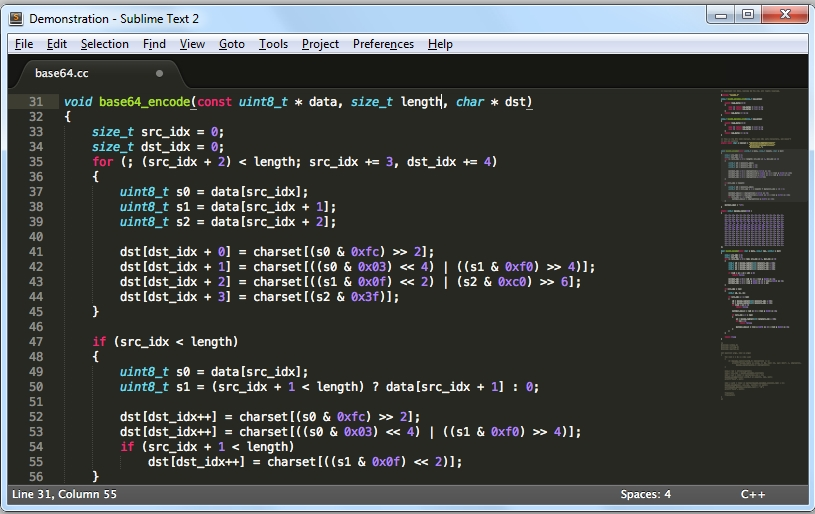
\includegraphics[width=1\textwidth]{./images/sublime.jpg}
	\rule{1\textwidth}{1pt}
	\caption{Sublime Text 2}
	\label{fig:sublime}
\end{figure}

\subsection{Git}
Git is a version control system (VCS) for tracking changes in computer files and coordinating work on those files among multiple people. It is primarily used for source code management in software development, but it can be used to keep track of changes in any set of files. As a distributed revision control system it is aimed at speed, data integrity, and support for distributed, non-linear workflows.
\newline

Git was created by Linus Torvalds in 2005 for development of the Linux kernel, with other kernel developers contributing to its initial development. Its current maintainer since 2005 is Junio Hamano.
\newline

As with most other distributed version control systems, and unlike most client–server systems, every Git directory on every computer is a full-fledged repository with complete history and full version tracking abilities, independent of network access or a central server.
\newline

Like the Linux kernel, Git is free software distributed under the terms of the GNU General Public License version 2.

\subsection{Eclipse}
\begin{figure}[h!]
	\centering
	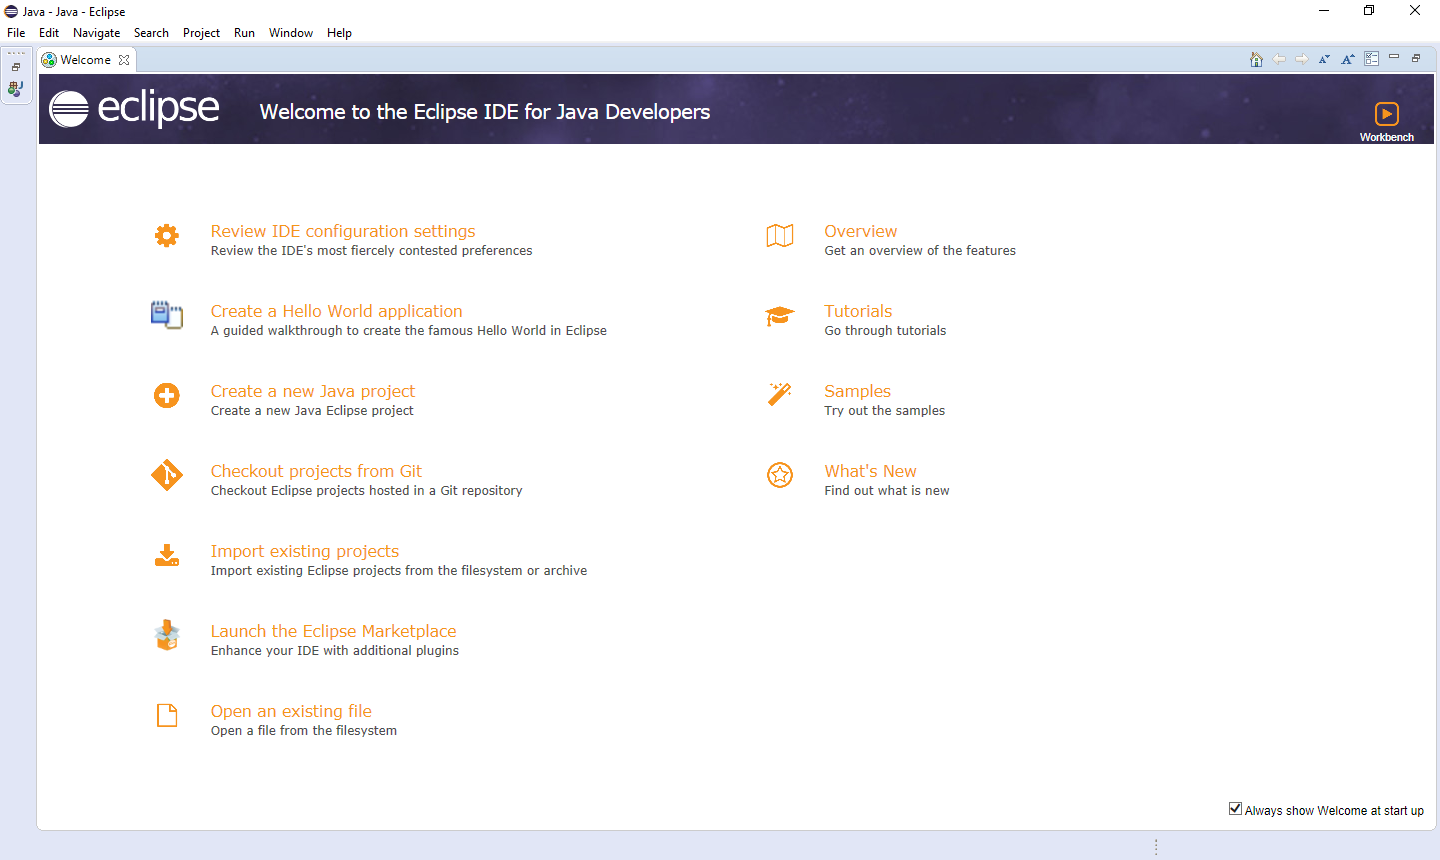
\includegraphics[width=1\textwidth]{./images/eclipse}
	\rule{1\textwidth}{1pt}
	\caption{Eclipse Welcome Screen}
	\label{fig:eclipse}
\end{figure}
Eclipse (Figure \ref{fig:eclipse}) is an integrated development environment (IDE) used in computer programming, and is the most widely used Java IDE. It contains a base workspace and an extensible plug-in system for customizing the environment. Eclipse is written mostly in Java and its primary use is for developing Java applications, but it may also be used to develop applications in other programming languages via plug-ins, including Ada, ABAP, C, C++, COBOL, D, Fortran, Haskell, JavaScript, Julia, Lasso, Lua, NATURAL, Perl, PHP, Prolog, Python, R, Ruby (including Ruby on Rails framework), Rust, Scala, Clojure, Groovy, Scheme, and Erlang. It can also be used to develop documents with LaTeX (via a TeXlipse plug-in) and packages for the software Mathematica. Development environments include the Eclipse Java development tools (JDT) for Java and Scala, Eclipse CDT for C/C++, and Eclipse PDT for PHP, among others.
\newline

The initial codebase originated from IBM VisualAge. The Eclipse software development kit (SDK), which includes the Java development tools, is meant for Java developers. Users can extend its abilities by installing plug-ins written for the Eclipse Platform, such as development toolkits for other programming languages, and can write and contribute their own plug-in modules. Since Equinox, plug-ins can be plugged-stopped dynamically and are termed (OSGI) bundles Eclipse software development kit (SDK) is free and open-source software, released under the terms of the Eclipse Public License, although it is incompatible with the GNU General Public License. It was one of the first IDEs to run under GNU Classpath and it runs without problems under IcedTea.

\subsection{PuTTY}
PuTTY (Figure \ref{fig:putty}) is a free and open-source terminal emulator, serial console and network file transfer application. It supports several network protocols, including SCP, SSH, Telnet, rlogin, and raw socket connection. It can also connect to a serial port (since version 0.59). The name "PuTTY" has no definitive meaning.
\newline

PuTTY was originally written for Microsoft Windows, but it has been ported to various other operating systems. Official ports are available for some Unix-like platforms, with work-in-progress ports to Classic Mac OS and Mac OS X, and unofficial ports have been contributed to platforms such as Symbian and Windows Mobile.
PuTTY was written and is maintained primarily by Simon Tatham and is currently beta software.
\begin{figure}[h!]
	\centering
	\vspace{-0.2cm}
	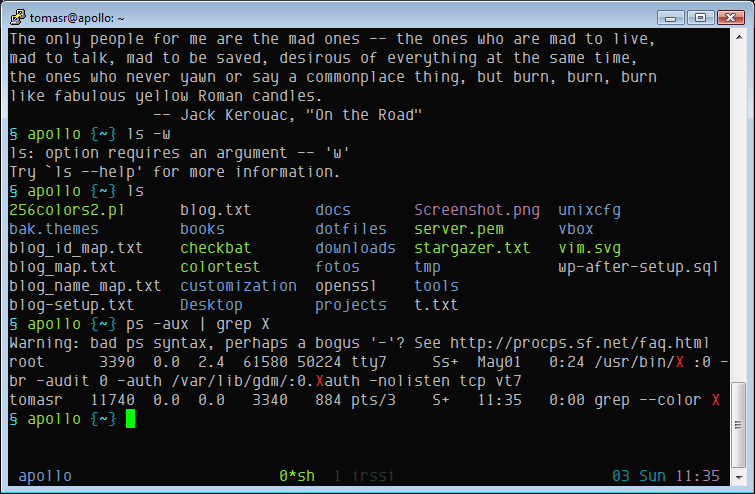
\includegraphics[width=0.8\textwidth]{./images/putty_tango.png}
	\rule{1\textwidth}{1pt}
	\caption{Putty interface}
	\label{fig:putty}
\end{figure}
%\clearpage
%----------------------------------------------------------------------------------------
%	Hardware
%----------------------------------------------------------------------------------------
\newline


\section{Hardware}

\begin{wrapfigure}{r}{0.3\textwidth}
	\begin{center}
		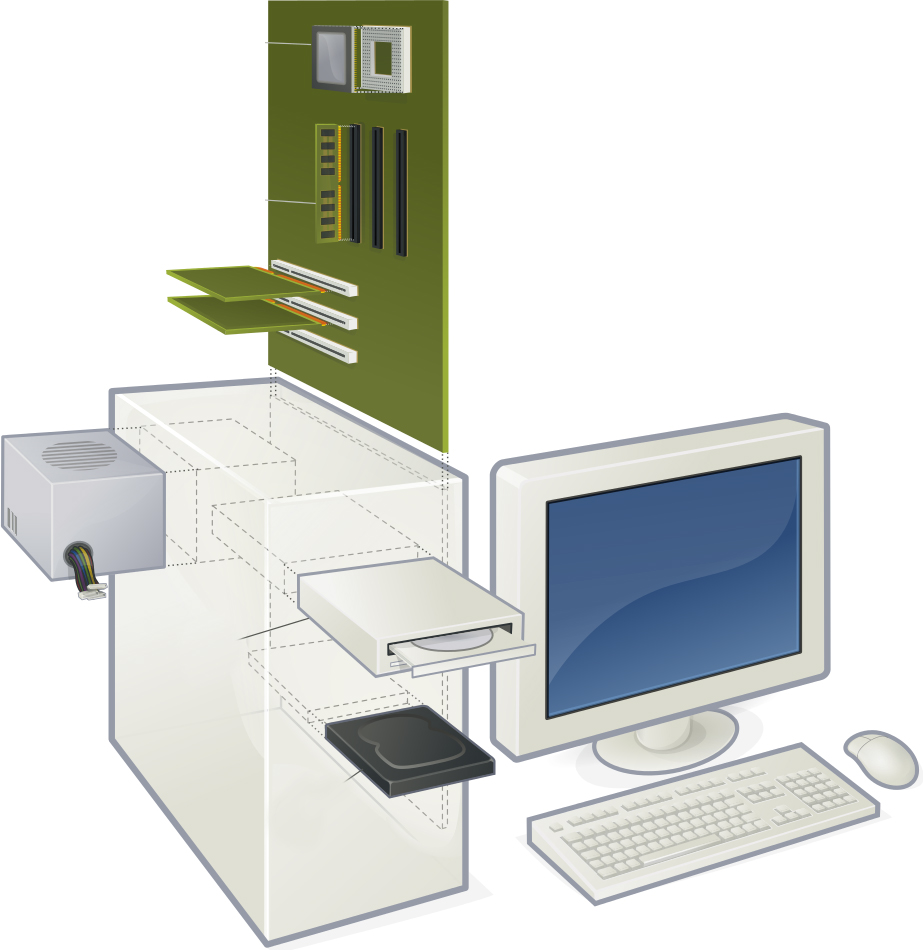
\includegraphics[width=0.3\textwidth]{./images/hardware.jpg}
	\end{center}
	\rule{0.3\textwidth}{0.5pt}
	\caption{Hardware of a modern personal computer}
	\label{fig:hardware}
\end{wrapfigure}

Computer hardware is the collection of physical parts of a computer system. This includes the computer case, monitor, keyboard, and mouse. It also includes all the parts inside the computer case, such as the hard disk drive, motherboard, video card, and many others. Computer hardware is what you can physically touch.[\cite{21}]
\subparagraph*{Definitions}
\hfill \break
A computer system consists of two major elements: hardware and software. Computer hardware is the collection of all the parts you can physically touch. Computer software, on the other hand, is not something you can touch. Software is a set of instructions for a computer to perform specific operations. You need both hardware and software for a computer system to work.

Some hardware components are easy to recognize, such as the computer case, keyboard, and monitor. However, there are many different types of hardware components. In this lesson, you will learn how to recognize the different components and what they do.[\cite{20}]
%-----------------------------------
%	SUBSECTION 1
%-----------------------------------
\subsection{Xiaomi Mi Band}

The Xiaomi Mi Band\footnote{\href{http://www.mi.com/en/miband/}{\texttt{http://www.mi.com/en/miband/}}} (Figure \ref{fig:smartband}) is a wearable fitness tracker produced by Xiaomi. Xiaomi Mi Band was unveiled during a Xiaomi launch event on 22 July 2014.
\begin{figure}[h]
	\centering
	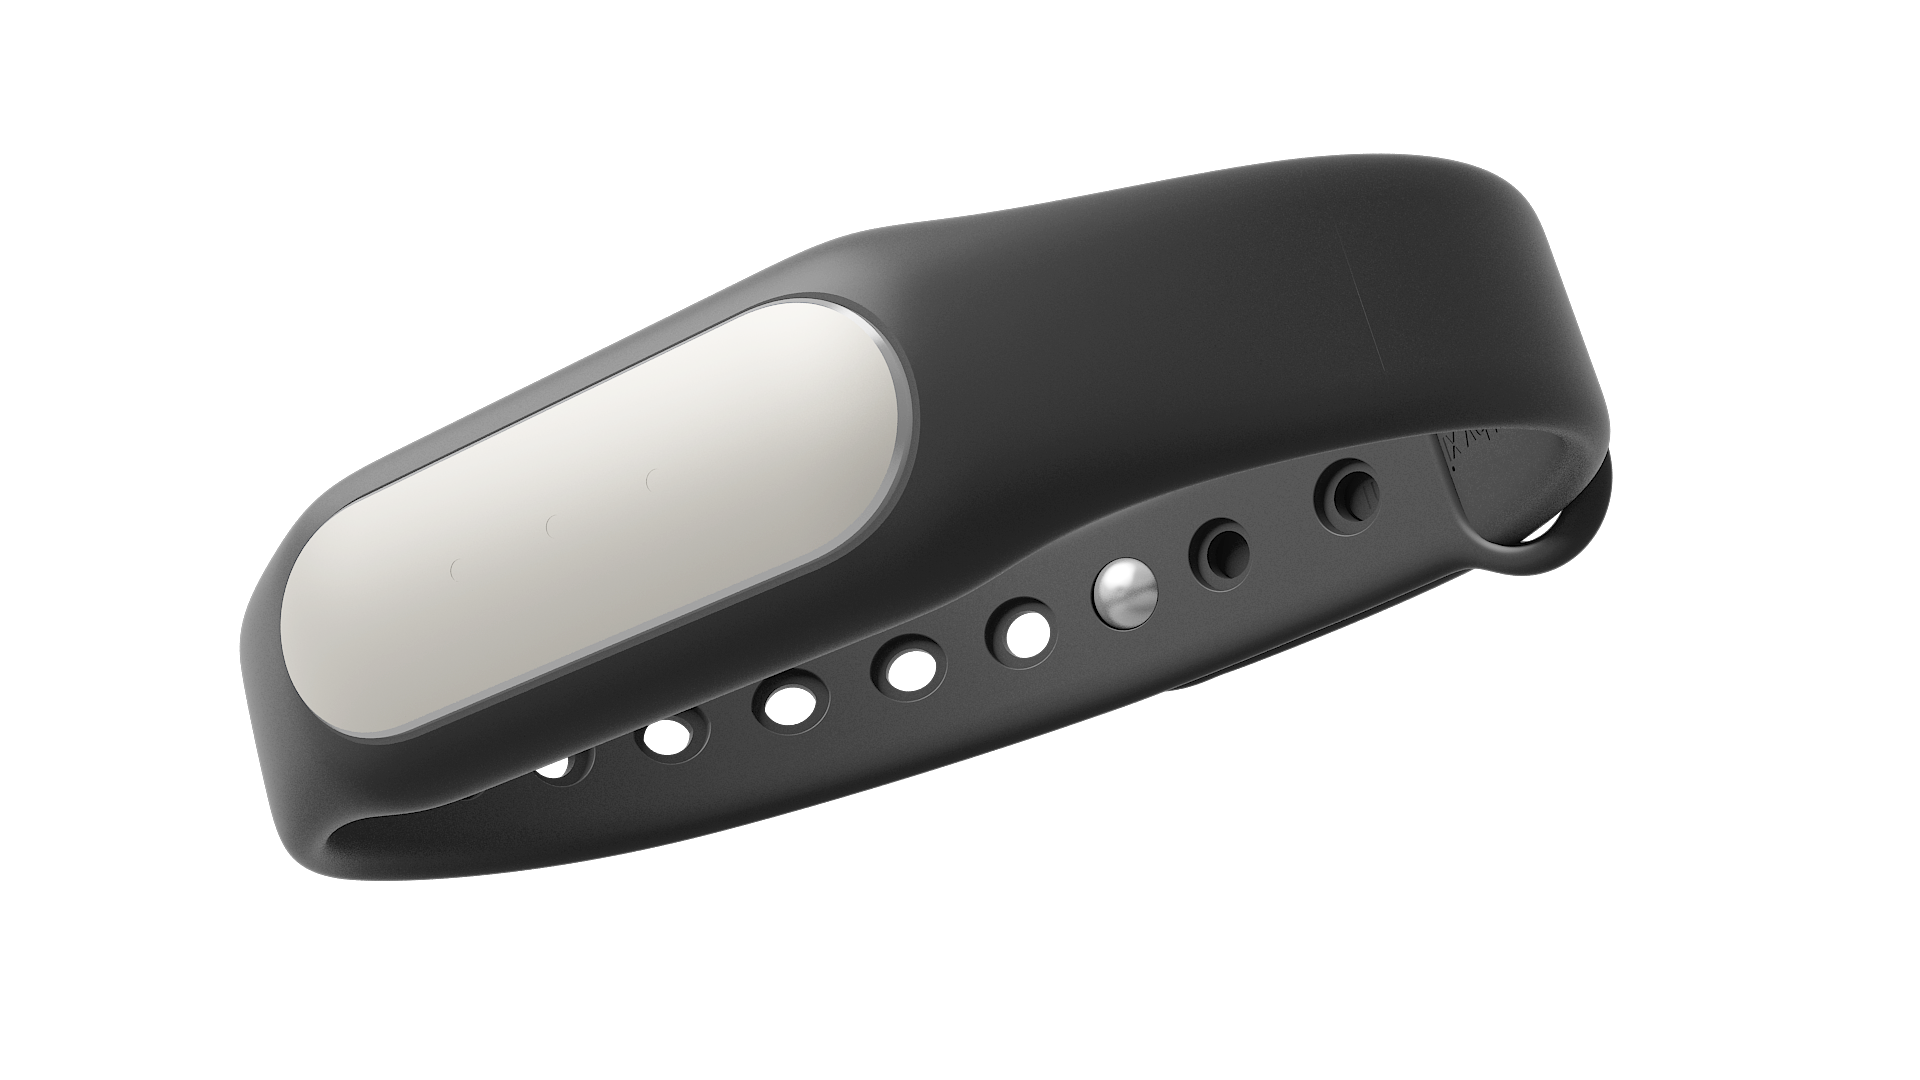
\includegraphics[width=0.7\linewidth]{images/smartband}
	\caption{Xiaomi Mi Band}
	\label{fig:smartband}
\end{figure}

Specifications:
\begin{itemize}
	\item Fitness monitor \& sleep tracker
	\item Sleep-cycle smart alarm
	\item Unlock your Android without a password
	\item 30-day standby power
	\item Water resistant (IP67)
	\item vibrate alert(call \& notification)
\end{itemize}

%-----------------------------------
%	SUBSECTION 2
%-----------------------------------
\subsection{Raspberry Pi}

The Raspberry Pi[\footnote{\href{https://www.raspberrypi.org/help/what-is-a-raspberry-pi/}{\texttt{https://www.raspberrypi.org/help/what-is-a-raspberry-pi/}}}] (Figure \ref{fig:raspberry})  is a series of small single-board computers developed in the United Kingdom by the Raspberry Pi Foundation to promote the teaching of basic computer science in schools and in developing countries. The original model became far more popular than anticipated, selling outside of its target market for uses such as robotics. Peripherals (including keyboards, mice and cases) are not included with the Raspberry Pi. Some accessories however have been included in several official and unofficial bundles.
\newline
\begin{figure}[h]
	\centering
	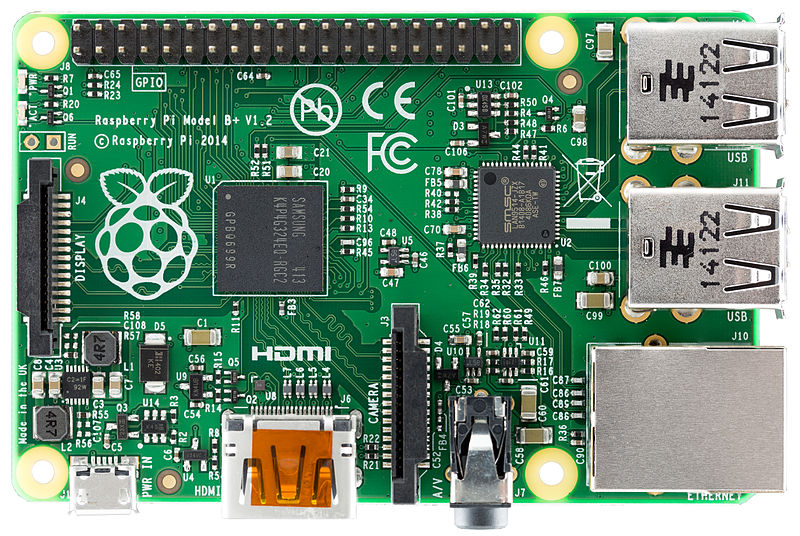
\includegraphics[width=0.5\linewidth]{images/raspberrypi.jpg}
	\caption{Raspberry Pi 1 model B+}
	\label{fig:raspberry}
\end{figure}

Over the past decades, computers have gotten cheaper and cheaper, so today
you can find them not only at your desk, but also in nearly every consumer
electronics device, such as smartphones and DVD players. Still, computers
aren’t so cheap that you spontaneously buy one when shopping for your
groceries. Usually, you carefully plan your next computer purchase, because
you have to use it for a couple of years.
\newline

Computers like the Raspberry Pi will change the situation completely in the
near future. The Raspberry Pi or Pi, for short is a full-blown desktop PC
that costs only \$35. You can connect it directly to the Internet, and it can
display high-definition videos. Also, it runs Linux, so you don’t have to pay
for an operating system. This makes the Pi probably the first throwaway
computer in history.
\newline

Originally, the Raspberry Foundation  built the Pi to teach children how to
program, so it comes as no surprise that the Pi is an excellent device for
exactly this purpose. 
\newline

On top of that, you can use the Pi for many other
exciting things. For example, you can turn it into a multimedia center, use it as a cheap but powerful web server, or play some classic games.
\newline

The Pi is also a great machine for experimenting with electronics. In contrast
to many popular microcontroller boards, such as the Arduino, the Pi runs a
full-blown operating system, and you can choose from a wide range of programming
languages to implement your projects.
\newline

With cheap and small devices like the Raspberry Pi, a new era of ubiquitous
computing has begun, and you can be part of it.[\cite{21}]